
\FloatBarrier

\section{Система Ван-дер-Поля} %  % {{{1 _VDP_
\label{atu:sect:vdp}

\LinkRef{
  vdp: ASAU-16, 17(alt), ITMM-2011
}

\subsection{Определение системы и анализ её динамики} %  % {{{2 _vdp_task

% TODO: dyn_sys_chaos, chaos_in_phase_dyn_VDP_modul_dobr.pdf buffer_phemon_vdp

Модель нелинейной автоколебательной системы Ван-Дер-Поля~(\ref{atu:eq:vdp})
широко используется при исследовании динамики
колебательных систем, в которых происходит восполнение
энергии системы из внешнего источника~\cite{anisch_nonlin_eff,magni_theory_dyn_chaos,atu_asau16}:
%
\begin{equation}
 \ddot{x} - \varepsilon (1-x^2)  \dot{x} + \Omega_0^2 x  = u(t) .
\label{atu:eq:vdp}
\end{equation}
\noindent
где
\(x(t)\) -- координата колебаний,
\( \varepsilon \) -- параметр, определяющий получение
  энергии системой,
\( \Omega_0 \) -- собственная частота при \( \varepsilon = 0 \),
\(u(t)\) -- внешнее возмущающее воздействие.

При \( \varepsilon > 0 \) и \( u(t) = 0 \)
рассматриваемая система реализует режим автоколебаний
с постоянной частотой, зависящей от \( \varepsilon \):
%
\begin{equation}
\Omega \approx \Omega_0 \sqrt{ 1 - \left( \frac{\varepsilon}{2 \Omega_0} \right)^2 }.
\label{atu:eq:vdp_Omega}
\end{equation}

При этом амплитуда колебаний остаётся практически постоянной,
а сама форма колебаний принимает всё более нелинейный характер.

Под воздействием входного гармонического сигнала
\( u(t) = U_{in} \sin ( \omega_{in} t ) \)
система~(\ref{atu:eq:vdp}) может проявлять регулярную, сложно-периодическую
и хаотическую динамику.

Идентифицируемый параметр \( \varepsilon \)
характеризует поступление энергии в систему.
При $x \approx 0$ членом с $x^2$ можно пренебречь,
и нелинейность вырождается в ``отрицательное трение''.
При больших амплитудах колебаний член с $x^2$
начинает преобладать, там самым ограничивая рост амплитуды.

При анализе численного моделирования системы~(\ref{atu:eq:vdp})
следует осторожно относится к выводам о типе динамики,
которые можно сделать, исходя из фазового или расширенного фазового портрета.
Например, на рис.~\ref{atu:f:vdp_phase_f_reg},
при условиях
$ \varepsilon=1.50$, $U_{in}=0.3$, $\omega_{in}=0.27$
на левом графике
фазовая траектория получается плотной,
однако спектр свидетельствует о регулярной динамике
с ограниченным набором частот.

\begin{figure}[ht!]
\begin{center}
  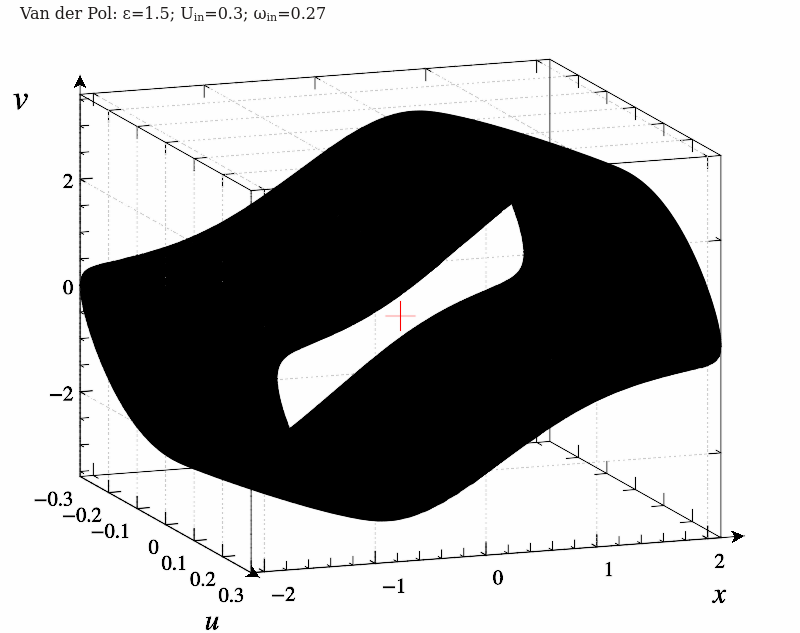
\includegraphics[width=0.49\textwidth]{p/cha/vdp/vdp_0-p_ph2d_1x50_0x30_0x27.png}
  \hfill
  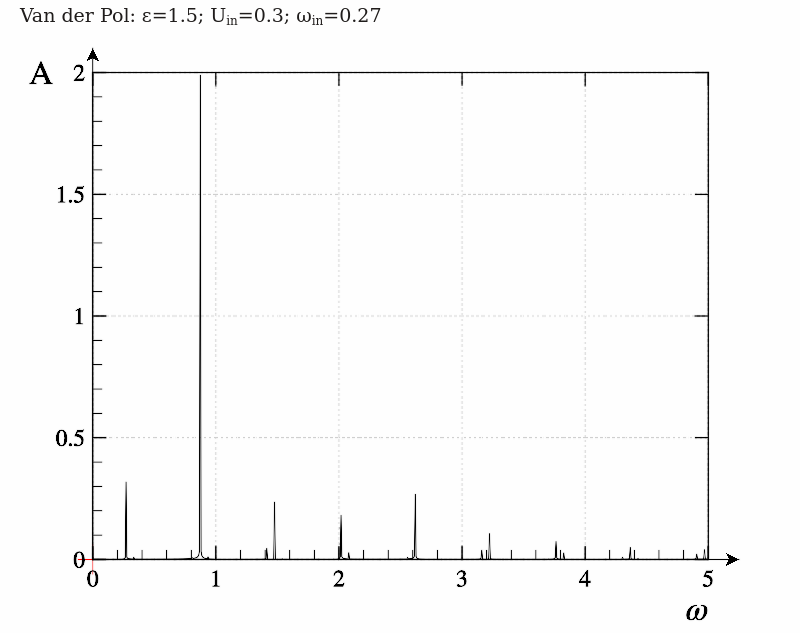
\includegraphics[width=0.49\textwidth]{p/cha/vdp/vdp_fft-p_f_1x50_0x30_0x27.png}
\end{center}
  \caption{Расширенный фазовый портрет и спектр системы Ван-дер-Поля (\ref{atu:eq:vdp}) в режиме регулярных колебаний}
\label{atu:f:vdp_phase_f_reg}
\end{figure}

Непосредственно хаотические колебания этой системы часто характеризуются
менее выраженной плотностью аттрактора. Тем не менее,
участки сложного спектра (рис.~\ref{atu:f:vdp_phase_f_chaos})
свидетельствуют в пользу хаоса.
Данная иллюстрация соответствует условиям
$ \varepsilon=2.65$, $U_{in}=1.2$, $\omega_{in}=0.27$.
При этом малые изменения параметров, например
снижение величины $\varepsilon$ до $2.5$
приводит к реализации режима простых регулярных колебаний.

\begin{figure}[ht!]
\begin{center}
  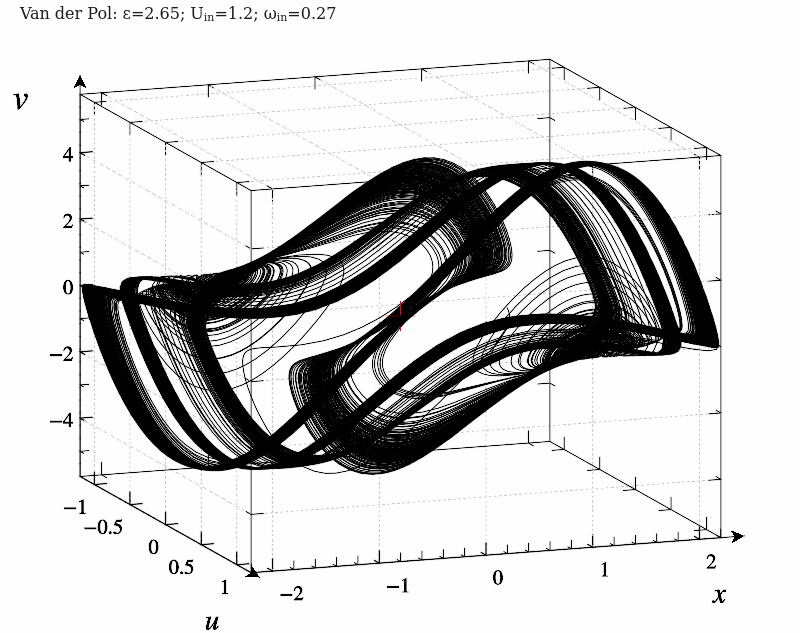
\includegraphics[width=0.49\textwidth]{p/cha/vdp/vdp_0-p_ph2d_2x65_1x20_0x27.png}
  \hfill
  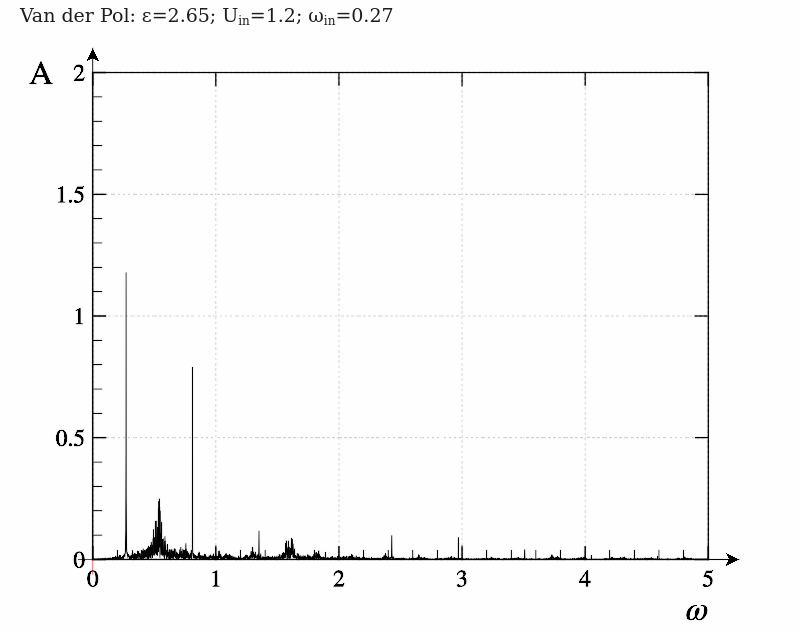
\includegraphics[width=0.49\textwidth]{p/cha/vdp/vdp_fft-p_f_2x65_1x20_0x27.png}
\end{center}
  \caption{Расширенный фазовый портрет и спектр системы Ван-дер-Поля (\ref{atu:eq:vdp}) в режиме хаотических колебаний}
\label{atu:f:vdp_phase_f_chaos}
\end{figure}

Анализ спектра системы Ван-дер-Поля, как и многих других систем
динамического хаоса, следует проводить, учитывая
спектральное разрешение.
Например, на  рис.~\ref{atu:f:vdp_phase_f_complex}
представлены результаты моделирования системы при
$ \varepsilon=4.8$, $U_{in}=0.7$, $\omega_{in}=0.7$.
С спектре системы наблюдаются участки с очень близко
расположенными пиками. При недостаточной разрешающей способности,
этот участок будет принят за зону сплошного спектра.
Это может привести к выводу о хаотичности системы,
тем более, если учесть вида аттрактора.

\begin{figure}[ht!]
\begin{center}
  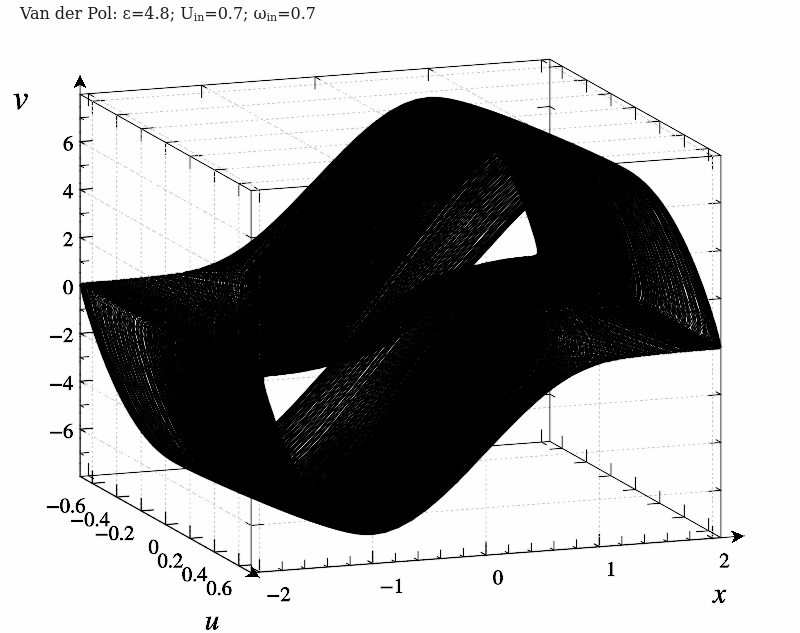
\includegraphics[width=0.49\textwidth]{p/cha/vdp/vdp_0-p_ph2d_4x80_0x70_0x70.png}
  \hfill
  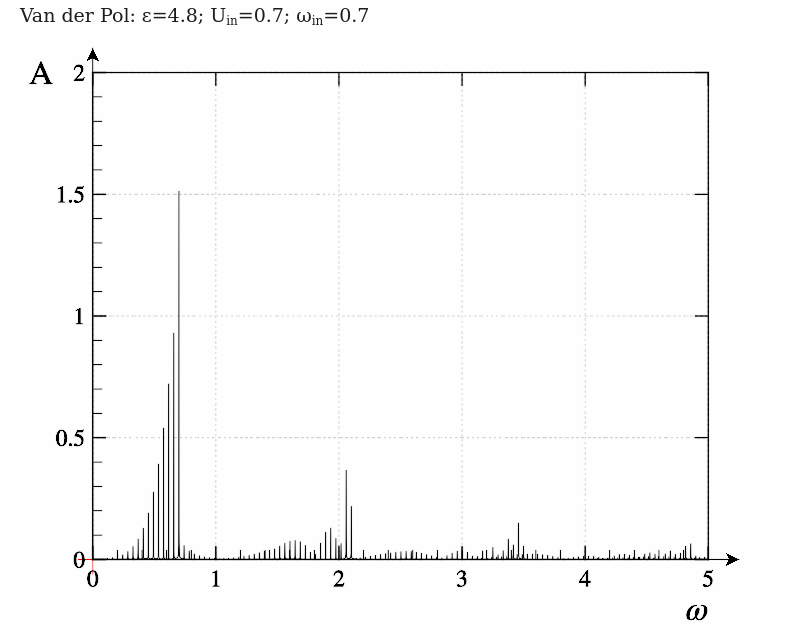
\includegraphics[width=0.49\textwidth]{p/cha/vdp/vdp_fft-p_f_4x80_0x70_0x70.png}
\end{center}
  \caption{Расширенный фазовый портрет и спектр системы Ван-дер-Поля (\ref{atu:eq:vdp}) в режиме сложных регулярных колебаний}
\label{atu:f:vdp_phase_f_complex}
\end{figure}


% \begin{figure}[htb!]
% \centerline{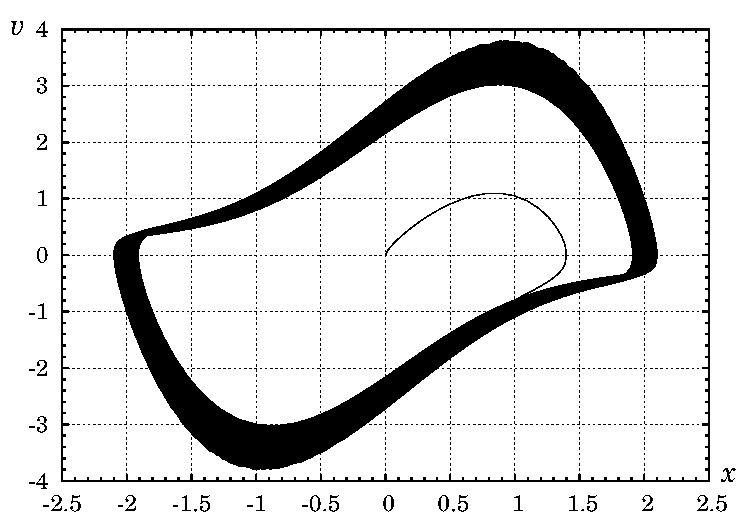
\includegraphics[width=0.5\textwidth]{p/cha/vdp_phase.pdf} }
% \caption{Фазовый портрет системы Ван-дер-Поля (\ref{atu:eq:vdp})}
% \label{atu:f:vdp_phase}
% \end{figure}

При анализе физических систем нет возможности произвольным образом
задавать время измерения для получения спектра с требуемым разрешением.
Более того, с учётом ограниченной точности измерений нет возможности
точно определить показатели Ляпунова. Таким образом,
вполне возможно существование систем, неотличимых от хаотических
при проведении измерений, но не являющимися хаотическими в строгом понимании.
Тем не менее, с точки зрения задачи идентификации,
этот случай практически неотличим от реального хаоса, и требует
применения соответствующих методов и критериев.

% }}}2


\subsection{Анализ и выбор критериев}  % {{{2

Критерий:
$\overline{T}$ + люфт + sign.

Альтернативный критерий:
$\overline{x^2}$

% }}}2

\subsection{Тестовая задача идентификации для системы Ван-дер-Поля}  % {{{2

% }}}2


\subsection{Влияние параметров системы идентификации на ошибку идентификации для системы Ван-дер-Поля}  % {{{2


Зависимости здесь

% }}}2

\subsection{Выводы}  % {{{2

Выводы

% }}}2



% }}}1

% vim: fdm=marker foldlevel=1 foldignore="%#" fdc=4 ft=tex
